\section{My\-Browser Class Reference}
\label{classMyBrowser}\index{MyBrowser@{MyBrowser}}
{\tt \#include $<$My\-Browser.h$>$}

Collaboration diagram for My\-Browser:\begin{figure}[H]
\begin{center}
\leavevmode
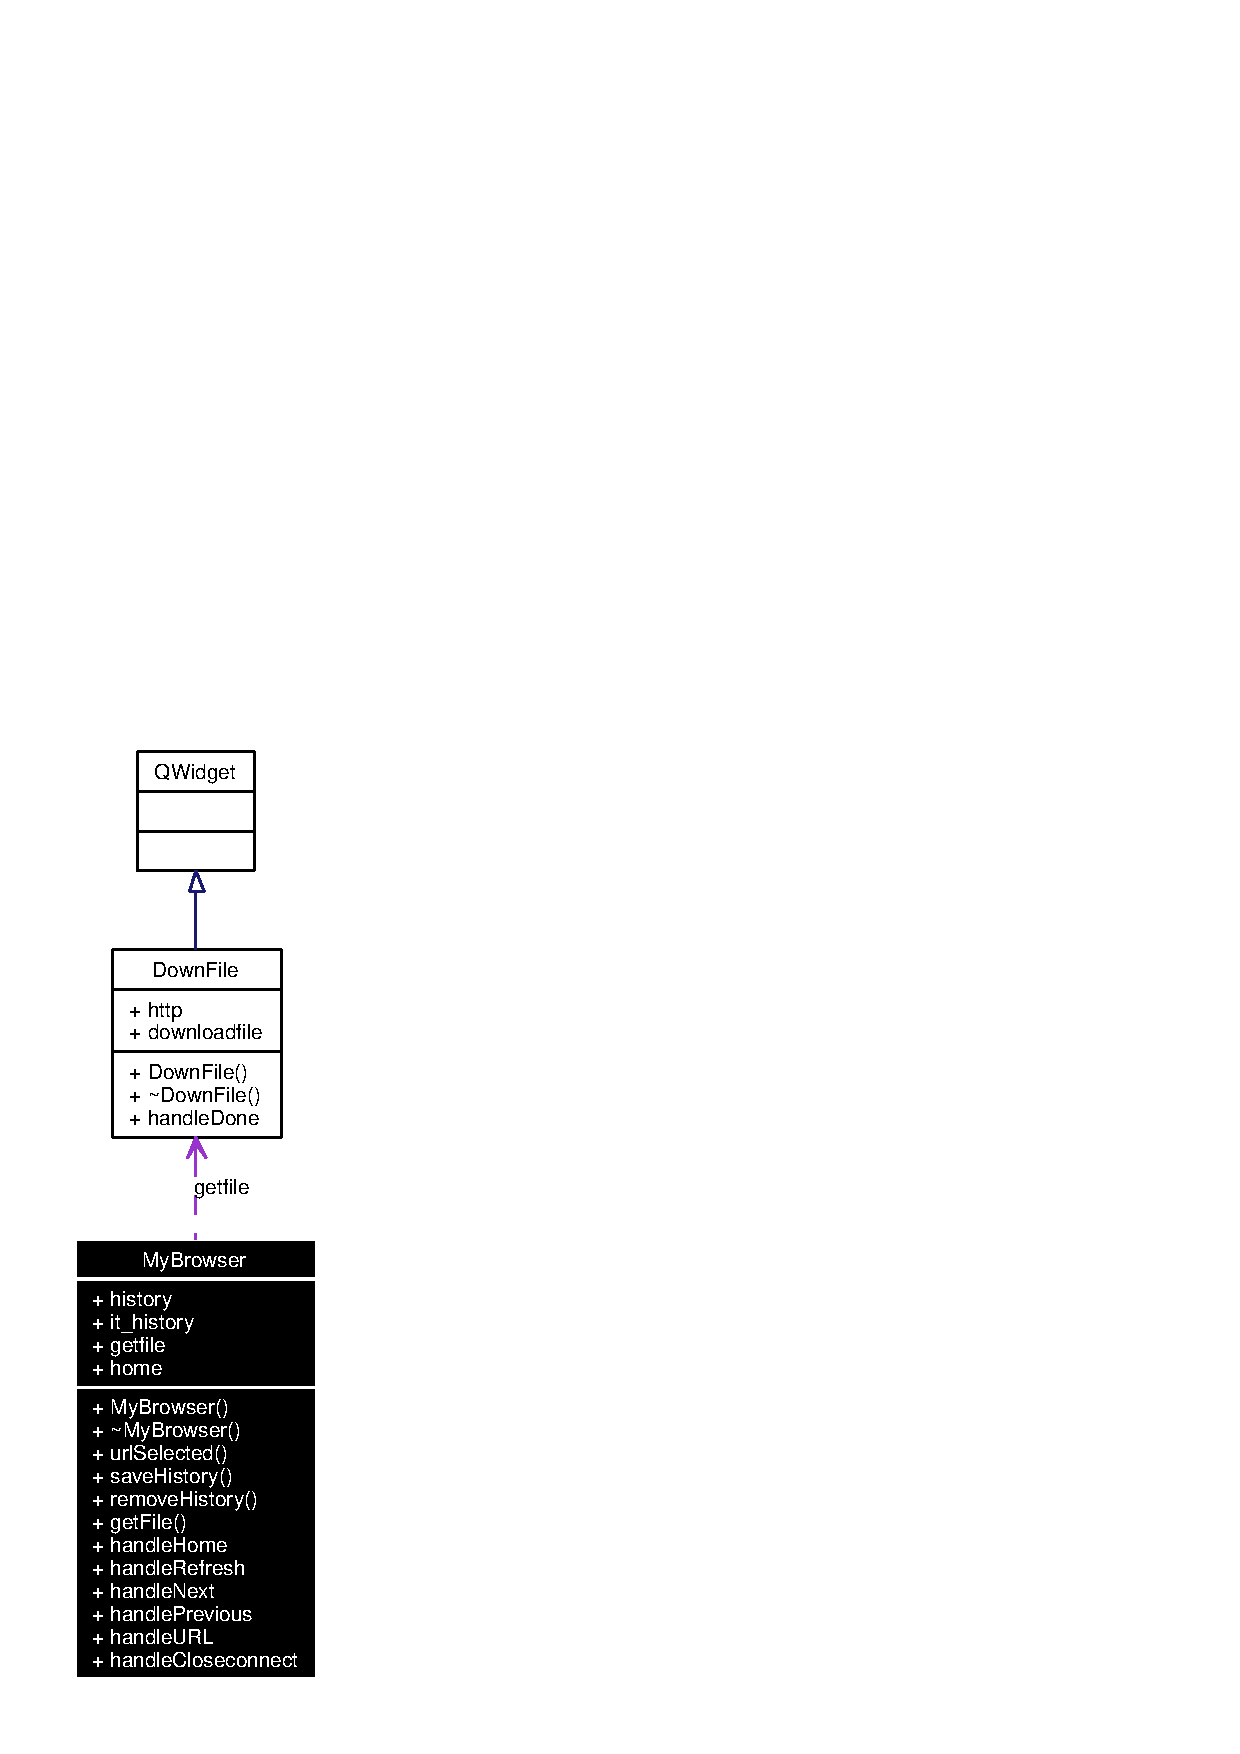
\includegraphics[width=76pt]{classMyBrowser__coll__graph}
\end{center}
\end{figure}
\subsection*{Public Slots}
\begin{CompactItemize}
\item 
void {\bf handle\-Home} ()
\item 
void {\bf handle\-Refresh} ()
\item 
void {\bf handle\-Next} ()
\item 
void {\bf handle\-Previous} ()
\item 
void {\bf handle\-URL} (const KURL \&, const KParts::URLArgs \&)
\item 
void {\bf handle\-Closeconnect} (bool)
\end{CompactItemize}
\subsection*{Public Member Functions}
\begin{CompactItemize}
\item 
{\bf My\-Browser} ({\bf QWidget} $\ast$parent\-Widget=0)
\item 
{\bf $\sim$My\-Browser} ()
\item 
void {\bf url\-Selected} (const QString \&url, int button, int state, const QString \&\_\-target, KParts::URLArgs args=KParts::URLArgs())
\item 
void {\bf save\-History} (const KURL \&)
\item 
void {\bf remove\-History} ()
\item 
void {\bf get\-File} (KURL \&)
\end{CompactItemize}
\subsection*{Public Attributes}
\begin{CompactItemize}
\item 
KURL::List {\bf history}
\item 
KURL::List::Iterator {\bf it\_\-history}
\item 
{\bf Down\-File} $\ast$ {\bf getfile}
\item 
KURL {\bf home}
\end{CompactItemize}


\subsection{Constructor \& Destructor Documentation}
\index{MyBrowser@{My\-Browser}!MyBrowser@{MyBrowser}}
\index{MyBrowser@{MyBrowser}!MyBrowser@{My\-Browser}}
\subsubsection{\setlength{\rightskip}{0pt plus 5cm}My\-Browser::My\-Browser ({\bf QWidget} $\ast$ {\em parent\-Widget} = 0)}\label{classMyBrowser_MyBrowsera0}




Definition at line 28 of file My\-Browser.cpp.

References handle\-Home(), history, home, and it\_\-history.



\footnotesize\begin{verbatim}29 : KHTMLPart(parentWidget)
30 {
31     it_history = history.begin();
32     home = KURL("http://tw.yahoo.com");
33     #if TRACE 
34     kdDebug() << "init() -> "<< home << endl;    
35     #endif
36     handleHome();      
37 }
\end{verbatim}\normalsize 
\index{MyBrowser@{My\-Browser}!~MyBrowser@{$\sim$MyBrowser}}
\index{~MyBrowser@{$\sim$MyBrowser}!MyBrowser@{My\-Browser}}
\subsubsection{\setlength{\rightskip}{0pt plus 5cm}My\-Browser::$\sim${\bf My\-Browser} ()}\label{classMyBrowser_MyBrowsera1}




Definition at line 40 of file My\-Browser.cpp.



\footnotesize\begin{verbatim}41 {
42 
43 }
\end{verbatim}\normalsize 


\subsection{Member Function Documentation}
\index{MyBrowser@{My\-Browser}!getFile@{getFile}}
\index{getFile@{getFile}!MyBrowser@{My\-Browser}}
\subsubsection{\setlength{\rightskip}{0pt plus 5cm}void My\-Browser::get\-File (KURL \&)}\label{classMyBrowser_MyBrowsera5}




Definition at line 84 of file My\-Browser.cpp.

References getfile, and handle\-Closeconnect().

Referenced by handle\-URL(), and url\-Selected().



\footnotesize\begin{verbatim}85 {
86 #if TRACE 
87 kdDebug()<< "getFile -> download a mp3 file "<< endl;
88 #endif
89     getfile = new DownFile(url);
90     connect(getfile,SIGNAL(Finished(bool)),this,SLOT(handleCloseconnect(bool)));
91 }
\end{verbatim}\normalsize 
\index{MyBrowser@{My\-Browser}!handleCloseconnect@{handleCloseconnect}}
\index{handleCloseconnect@{handleCloseconnect}!MyBrowser@{My\-Browser}}
\subsubsection{\setlength{\rightskip}{0pt plus 5cm}void My\-Browser::handle\-Closeconnect (bool)\hspace{0.3cm}{\tt  [slot]}}\label{classMyBrowser_MyBrowseri5}




Definition at line 157 of file My\-Browser.cpp.

References getfile.

Referenced by get\-File().



\footnotesize\begin{verbatim}158 {
159     delete getfile;
160     #if TRACE     
161 kdDebug() << "MyBrowser::handleCloseconnect -> Delete connection !!!!"<< endl;
162 #endif    
163 }
\end{verbatim}\normalsize 
\index{MyBrowser@{My\-Browser}!handleHome@{handleHome}}
\index{handleHome@{handleHome}!MyBrowser@{My\-Browser}}
\subsubsection{\setlength{\rightskip}{0pt plus 5cm}void My\-Browser::handle\-Home ()\hspace{0.3cm}{\tt  [slot]}}\label{classMyBrowser_MyBrowseri0}




Definition at line 95 of file My\-Browser.cpp.

References home, and save\-History().

Referenced by My\-Browser().



\footnotesize\begin{verbatim}96 {
97     if(home.protocol()=="http")
98     {
99         openURL(home);
100         saveHistory(home);
101     }   
102     else kdDebug() << "=====================Home -> " << home.protocol() << endl;
103 }
\end{verbatim}\normalsize 
\index{MyBrowser@{My\-Browser}!handleNext@{handleNext}}
\index{handleNext@{handleNext}!MyBrowser@{My\-Browser}}
\subsubsection{\setlength{\rightskip}{0pt plus 5cm}void My\-Browser::handle\-Next ()\hspace{0.3cm}{\tt  [slot]}}\label{classMyBrowser_MyBrowseri2}




Definition at line 105 of file My\-Browser.cpp.

References history, and it\_\-history.



\footnotesize\begin{verbatim}106 {
107 #if TRACE 
108 kdDebug() << "handleNext"<< endl;
109 #endif
110     if(it_history != history.end())
111     {
112         ++it_history;
113         openURL((*it_history).url());
114 
115     }   
116 }
\end{verbatim}\normalsize 
\index{MyBrowser@{My\-Browser}!handlePrevious@{handlePrevious}}
\index{handlePrevious@{handlePrevious}!MyBrowser@{My\-Browser}}
\subsubsection{\setlength{\rightskip}{0pt plus 5cm}void My\-Browser::handle\-Previous ()\hspace{0.3cm}{\tt  [slot]}}\label{classMyBrowser_MyBrowseri3}




Definition at line 118 of file My\-Browser.cpp.

References history, and it\_\-history.



\footnotesize\begin{verbatim}119 {
120 #if TRACE 
121 kdDebug() << "handlePrevious"<< endl;
122 #endif
123     if(it_history != history.begin())
124     {
125         --it_history;
126         openURL((*it_history).url());
127 
128     }   
129 }
\end{verbatim}\normalsize 
\index{MyBrowser@{My\-Browser}!handleRefresh@{handleRefresh}}
\index{handleRefresh@{handleRefresh}!MyBrowser@{My\-Browser}}
\subsubsection{\setlength{\rightskip}{0pt plus 5cm}void My\-Browser::handle\-Refresh ()\hspace{0.3cm}{\tt  [slot]}}\label{classMyBrowser_MyBrowseri1}




Definition at line 131 of file My\-Browser.cpp.



\footnotesize\begin{verbatim}132 {
133 #if TRACE 
134 kdDebug() << "handleRefresh"<< endl;
135 #endif    
136     openURL((*it_history).url());
137 }
\end{verbatim}\normalsize 
\index{MyBrowser@{My\-Browser}!handleURL@{handleURL}}
\index{handleURL@{handleURL}!MyBrowser@{My\-Browser}}
\subsubsection{\setlength{\rightskip}{0pt plus 5cm}void My\-Browser::handle\-URL (const KURL \&, const KParts::URLArgs \&)\hspace{0.3cm}{\tt  [slot]}}\label{classMyBrowser_MyBrowseri4}




Definition at line 139 of file My\-Browser.cpp.

References get\-File(), remove\-History(), and save\-History().



\footnotesize\begin{verbatim}140 {
141 #if TRACE 
142 kdDebug() << "handleURL -> submit control"<< endl;
143 #endif
144     if(uurl.protocol()=="http")
145     {
146         removeHistory();
147         openURL(uurl);
148         saveHistory(uurl);
149     }   
150     else if(uurl.protocol()=="hdas")
151     {           
152         KURL url = uurl;
153         getFile(url);
154     }
155 }
\end{verbatim}\normalsize 
\index{MyBrowser@{My\-Browser}!removeHistory@{removeHistory}}
\index{removeHistory@{removeHistory}!MyBrowser@{My\-Browser}}
\subsubsection{\setlength{\rightskip}{0pt plus 5cm}void My\-Browser::remove\-History ()}\label{classMyBrowser_MyBrowsera4}




Definition at line 75 of file My\-Browser.cpp.

References history, and it\_\-history.

Referenced by handle\-URL(), and url\-Selected().



\footnotesize\begin{verbatim}76 {
77     if(it_history != history.end())
78     {
79         KURL::List::Iterator it_remove = history.end();
80         for(it_remove;it_remove!=it_history;it_remove--)history.remove((*it_remove).url());
81     }
82 }
\end{verbatim}\normalsize 
\index{MyBrowser@{My\-Browser}!saveHistory@{saveHistory}}
\index{saveHistory@{saveHistory}!MyBrowser@{My\-Browser}}
\subsubsection{\setlength{\rightskip}{0pt plus 5cm}void My\-Browser::save\-History (const KURL \&)}\label{classMyBrowser_MyBrowsera3}




Definition at line 66 of file My\-Browser.cpp.

References history, and it\_\-history.

Referenced by handle\-Home(), handle\-URL(), and url\-Selected().



\footnotesize\begin{verbatim}67 {
68 #if TRACE 
69 kdDebug() << "Saving History !!"<< endl;
70 #endif
71         history << url;      
72         ++it_history;
73 }
\end{verbatim}\normalsize 
\index{MyBrowser@{My\-Browser}!urlSelected@{urlSelected}}
\index{urlSelected@{urlSelected}!MyBrowser@{My\-Browser}}
\subsubsection{\setlength{\rightskip}{0pt plus 5cm}void My\-Browser::url\-Selected (const QString \& {\em url}, int {\em button}, int {\em state}, const QString \& {\em \_\-target}, KParts::URLArgs {\em args} = KParts::URLArgs())}\label{classMyBrowser_MyBrowsera2}




Definition at line 45 of file My\-Browser.cpp.

References get\-File(), remove\-History(), and save\-History().



\footnotesize\begin{verbatim}46 {
47      KURL cURL = completeURL(url);
48      #if TRACE 
49 kdDebug() << "urlSelect -> " << cURL << endl;     
50 #endif
51      if(cURL.protocol()=="http")
52      {
53         removeHistory();
54         openURL(cURL);
55         saveHistory(cURL);
56      }
57      else if(cURL.protocol()=="hdas")
58      {
59 #if TRACE      
60 kdDebug()<< "MyBrowser::urlSelected -> HDAS -> " << cURL << endl;
61 #endif
62         getFile(cURL);
63      }
64 }
\end{verbatim}\normalsize 


Here is the call graph for this function:\begin{figure}[H]
\begin{center}
\leavevmode
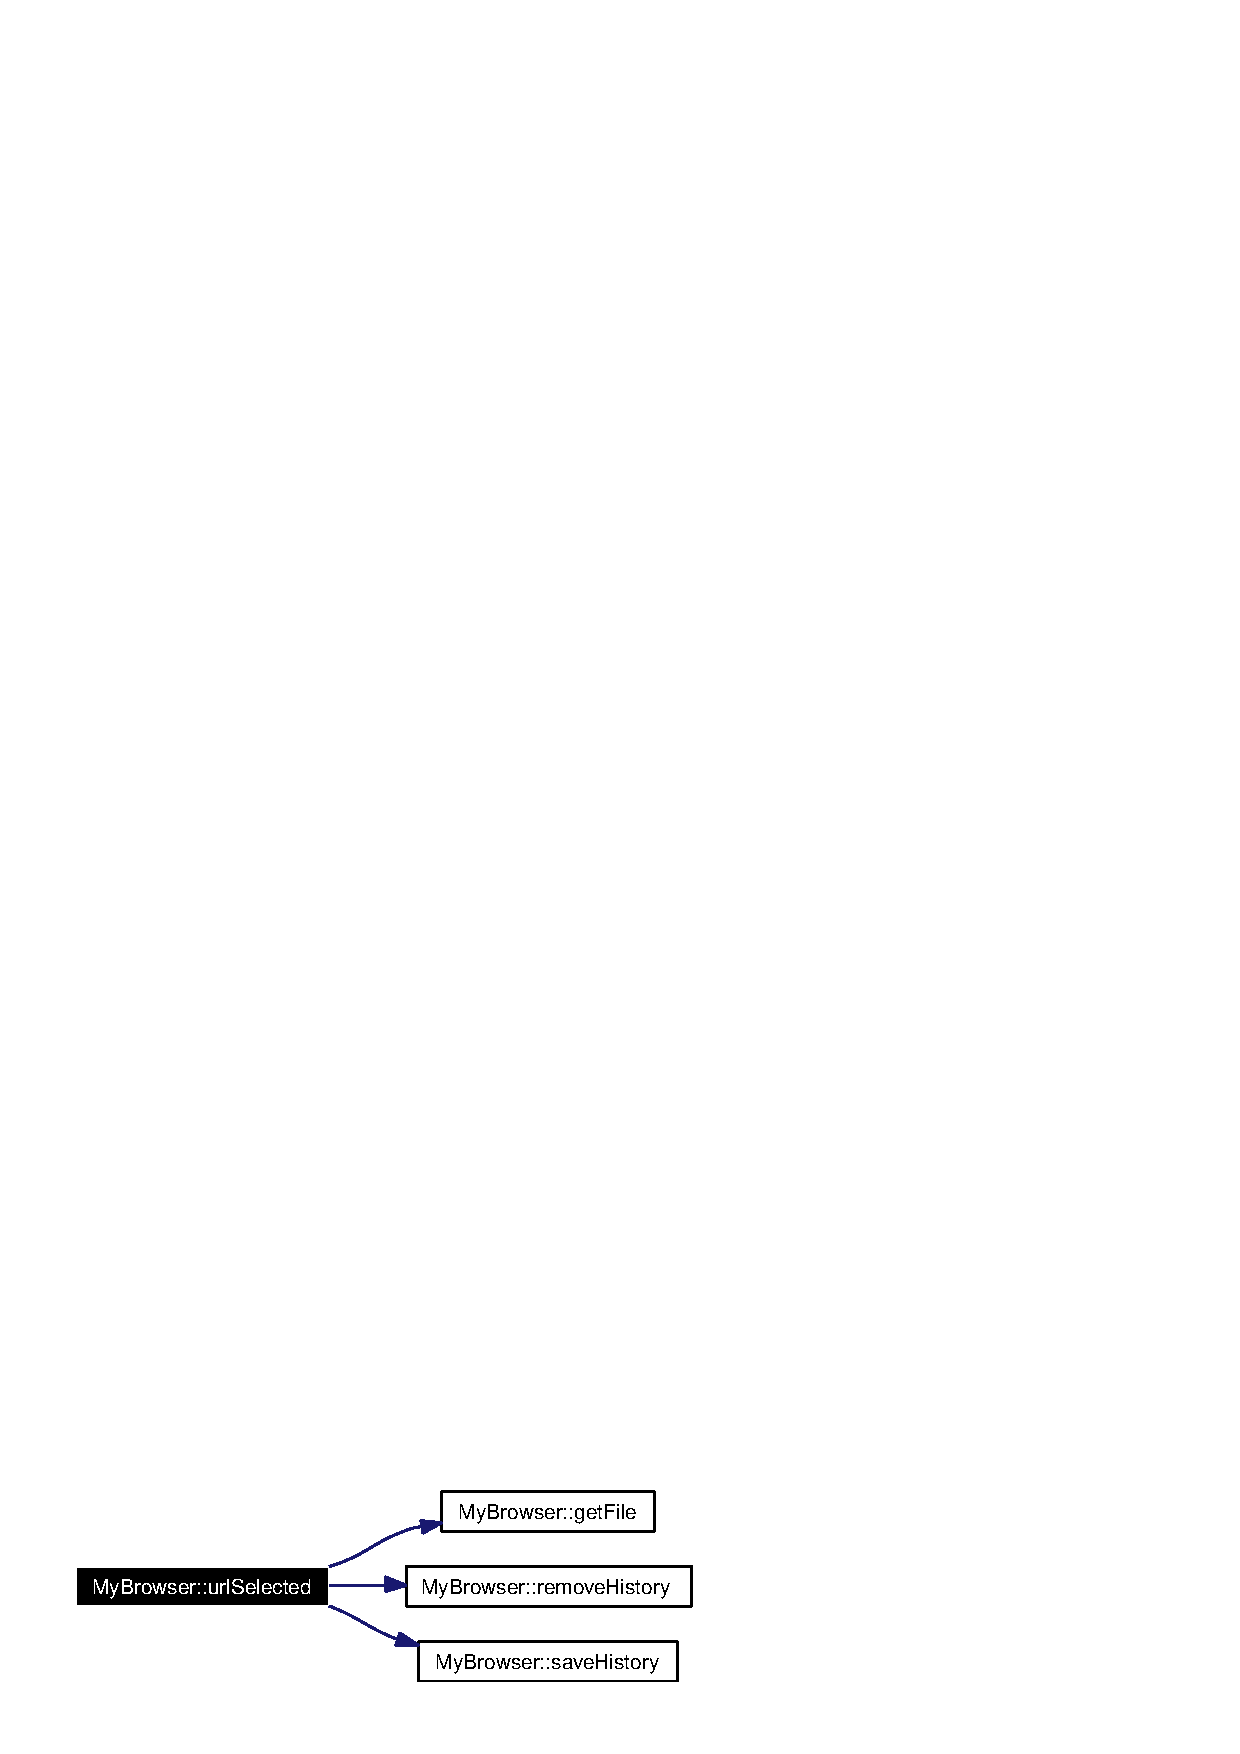
\includegraphics[width=166pt]{classMyBrowser_MyBrowsera2_cgraph}
\end{center}
\end{figure}


\subsection{Member Data Documentation}
\index{MyBrowser@{My\-Browser}!getfile@{getfile}}
\index{getfile@{getfile}!MyBrowser@{My\-Browser}}
\subsubsection{\setlength{\rightskip}{0pt plus 5cm}{\bf Down\-File}$\ast$ {\bf My\-Browser::getfile}}\label{classMyBrowser_MyBrowsero2}




Definition at line 45 of file My\-Browser.h.

Referenced by get\-File(), and handle\-Closeconnect().\index{MyBrowser@{My\-Browser}!history@{history}}
\index{history@{history}!MyBrowser@{My\-Browser}}
\subsubsection{\setlength{\rightskip}{0pt plus 5cm}KURL::List {\bf My\-Browser::history}}\label{classMyBrowser_MyBrowsero0}




Definition at line 43 of file My\-Browser.h.

Referenced by handle\-Next(), handle\-Previous(), My\-Browser(), remove\-History(), and save\-History().\index{MyBrowser@{My\-Browser}!home@{home}}
\index{home@{home}!MyBrowser@{My\-Browser}}
\subsubsection{\setlength{\rightskip}{0pt plus 5cm}KURL {\bf My\-Browser::home}}\label{classMyBrowser_MyBrowsero3}




Definition at line 46 of file My\-Browser.h.

Referenced by handle\-Home(), and My\-Browser().\index{MyBrowser@{My\-Browser}!it_history@{it\_\-history}}
\index{it_history@{it\_\-history}!MyBrowser@{My\-Browser}}
\subsubsection{\setlength{\rightskip}{0pt plus 5cm}KURL::List::Iterator {\bf My\-Browser::it\_\-history}}\label{classMyBrowser_MyBrowsero1}




Definition at line 44 of file My\-Browser.h.

Referenced by handle\-Next(), handle\-Previous(), My\-Browser(), remove\-History(), and save\-History().

The documentation for this class was generated from the following files:\begin{CompactItemize}
\item 
{\bf My\-Browser.h}\item 
{\bf My\-Browser.cpp}\end{CompactItemize}
